\section{Generierung}
\label{Generierung}
Bei der Generierung lautet die Aufgabe, aus den Klassenzuordnungen eines Zeitabschnitts wieder einen Lastgang zu erstellen. Es ist also die gegenteilige Aufgabe zur Klassifikation, statt aus einem Lastgang ein Zustandsprofil zu erstellen wird aus einem Zustandsprofil ein Lastgang erstellt.
Zusammen mit der Klassifikation und intelligenten Haushaltsger"aten k"onnen so Vorhersagen "uber den Verbrauch der Ger"ate getroffen werden und ein zentrales System kann die Nutzung der Ger"ate planen. \\

Ein Szenario: Die Waschmaschine hat die M"oglichkeit mit dem zentralen Planungssystem zu kommunizieren. In der Trainingsphase m"ussen zun"achst die Lastg"ange f"ur die unterschiedlichen Programme der Maschine aufgezeichnet und klassifiziert werden, so dass man anschlie{\ss}end ein Zustandsprofil f"ur jedes Programm hat. In einem normalen Haushalt mit Planungssystem kann die Waschmaschine dann dem System mitteilen, welches Zustandsprofil der Nutzer w"unscht und bis wann der Waschgang beendet sein soll, z.B. 30\celsius Buntw"asche bis 18.00. Das Planungssystem kann dann den Lastgang simulieren, die optimale Lage im gegebenen Zeitfenster bestimmen und dann die Waschmaschine informieren, wann sie waschen soll.
Die optimale Lage k"onnte sich in diesem Szenario z.B. durch einen flexiblen Energiepreis bestimmen. \\

Die f"ur ein solches Szenario n"otigen Zustandsprofile erstellt die Klassifikation automatisch, wichtig ist jedoch, dass die Energiedaten der Waschmaschine einzeln gemessen werden m"ussen, dies kann z.B. beim Hersteller oder in einem Labor geschehen. Das Planungssystem wird in dieser Arbeit nicht vollst"andig behandelt, es wird nur die Simulation des Lastgangs besprochen. \\

\subsection{Stand der Technik}
\label{Stand der Technik}
Das Konzept des L/H-converter aus \cite{hara2008multi} ist ein sehr allgemeines Konzept zum simulieren eines hoch aufgel"osten Signals aus einem niedrig aufgel"osten. Das Zustandsprofil stellt dabei das niedrig aufgel"oste Signal dar, der Wertebereich umfasst die Werte 0,1,2,3,4,5, w"ahrend die Wirkleistung als hoch aufgel"ostes Signal der kompletten Wertebereich von 0 bis 2200 Watt abdeckt. \cite{hara2008multi} gibt f"ur den L/H-converter folgende Formel an.\\
\begin{center}
$x_{high} = R^{L/H} x_{low}$
\end{center}
$R^{L/H}$ stellt dabei die Funktion zur Simulation dar, diese muss in der Implementierung spezifiziert werden.
Abbildung~\ref{converter} zeigt noch einmal die Einordnung des L/H-converter in einem System mit verschiedenen Aufl"osungen, wobei das Low Resolved System in unserem Fall das Zustandsprofil und das High Resolved System den Lastgang repr"asentiert. 
\begin{figure}[h]
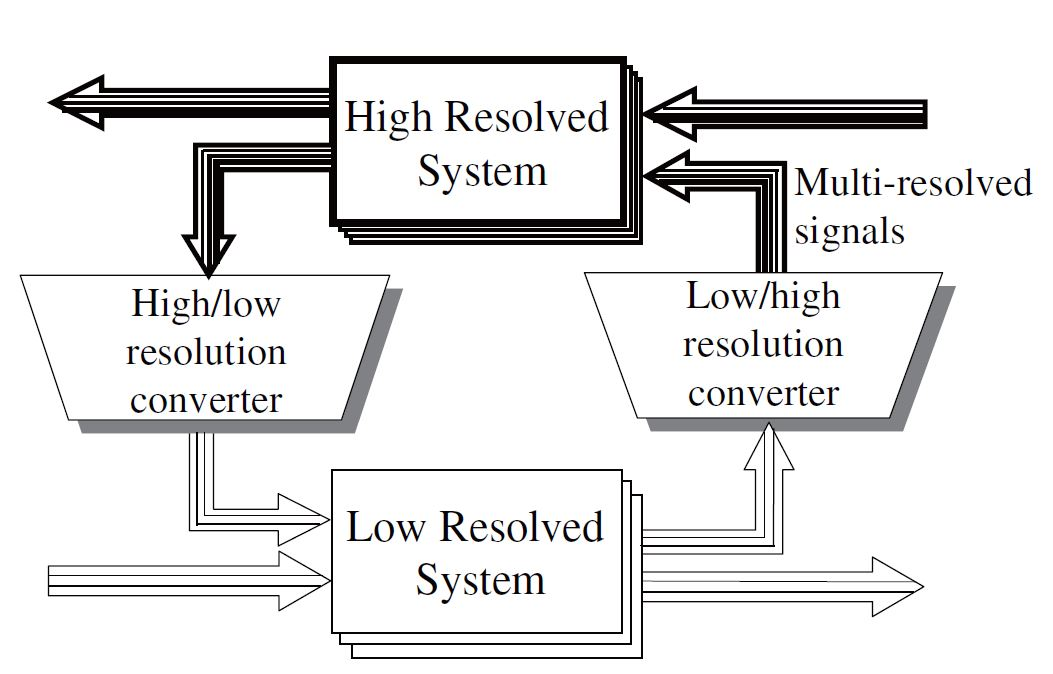
\includegraphics[height=0.7\textwidth]{1_Grafiken/multiresolved.jpg}
	\caption[Multi Resolved System]{Schematische Darstellung eines Systems mit verschiedenen Aufl"osungen und den Konvertern, die die Aufl"osung im Informationsfluss anpassen.}
\label{converter}
\end{figure}

\subsection{Vorgehensweise}
\label{Vorgehensweise}
Die Erstellung eines Lastgangs nur aufgrund des klassifizierten Zustands der Maschine ist nicht besonders sinnvoll, denn das neuronale Netz kann nach dem Training nur die Mittelwerte f"ur die Wirkleistung der einzelnen Klassen angeben und es entsteht ein unrealistischer, extrem glatter Lastgang. Die Verwendung einer Zeitreihe schafft einen wesentlich realistischeren Lastgang. Man kann sich hier zu nutze machen, dass man vor Beginn des Programms implizit annehmen kann, dass sich die Maschine im \textit{Off-Zustand} befindet. Man nimmt also f"ur den ersten zu simulierenden Wert des Waschgangs die vorherige Wirkleistung als 0 an und kann dann iterativ immer einen neuen Wert berechnen. F"ur die Simulation stehen dem Netz die Werte der Wirkleistung von $t-10$ bis $t-1$ und die Klasse von $t+0$ zur Verf"ugung.\\
\begin{center}
$t+0 = F(t-1,...,t-10,K(t+0))$
\end{center}
Die Funktion $F$ ist die Simulationsfunktion, in diesem Falls also das neuronale Netz und $K(t+0)$ ist die Klassifikation des des Zeitpunktes t+0. Der Rekursion von $F$ endet, wenn der Beginn des Waschgangs erreicht ist, dann gilt \\
\begin{center} 
$t+0 = F(t-1,...,t-10,K(t+0)) = F(0,...,0,K(t+0))\ f"ur\ t = 0$
\end{center} 
Bezogen auf die in \ref{Stand der Technik} gegebene Formel f"ur die Simulation gilt: $t+0\ \widehat{=}\ x_{high}\ , K(t+0)\ \widehat{=}\ x_{low}\ und\ F\ \widehat{=}\ R^{L/H}$